% Game engine arch
\chapter{Game engine architecture}

Game engines are tightly connected to the evolution of video games themselves. Where 50 years ago a game was build out of hardware the rapid development of a computer's processing power and storage capabilities changed the process of how games are made. Today a game runs on machines assembled from multiple cores, several \acp{GB} of \ac{RAM} and a powerful \ac{GPU}. But whether the target platform is a PC or a specialized gaming console every modern game has to fulfill certain constraints to be a viable product. This chapter will highlight some of the most important milestones in the history of video games and game engines. It will also give an overview of well-known products on the game engine market and will conclude with the description of selected submodules, the underlying building blocks of a game engine.

\section{Evolution of game engines}

When the first developers started to create video games, the term \textit{game engine} was non existent. At this time the software that ran the simulation a player experienced was tailored to the needs of a specific genre, hardware and game. It was then in the 1990s and with the rise of games like \textit{Doom (1993)} and \textit{Quake (1996)} that certain software was referred to as a \textit{game engine}. The mentioned games separated their technical backbones into different components, creating an architecture that distinguishes between core software modules and game specific entities such as art assets, levels and the general rules of the game. Due to the well-designed architecture and separations the effort to create a new game, where the general concept is the same, was reduced from writing every system and piece of code to creating new art and only tweak and configure the software of previous games. This was also the birth of the \textit{modding} community, where individuals and also studios modify existing games or engine software to create new content or whole games.

From that time on the developers created their games with modding and future extension in mind. Smaller studios started to license the parts of the engine software they could not afford to create by themselves, be it money, time or man power. With the concept of licensing studios, that created the extensible and reusable software packages, created another source of income. But while the goal of an extensible and reusable software collection is a desirable one, the line between a game and an engine is often softer than desired. Because of the nature of games and their specific genre rules it is hard, if not even impossible, to develop a generic engine that can serve as a template for every game. It became the responsibility of the engine developer to find the balance between general-purpose functionality and game or platform tailored optimizations. This trade-off has to be made because the developer can only assume how the software will be used. And so a game engine developed and optimized for rendering \acp{FPS} will probably not run a \ac{RTS} game with maximum performance due to the different rule sets and features both genres require.

Empowered by the wish of creating games that can be modded and licensed bigger studios started to create commercial engines. \textit{Id Software}, the company that created \textit{Doom} and the \textit{Quake} trilogy, opened up the field with their \ac{FPS} engines in the early 1990s. \textit{Id Software} was then followed by \textit{Epic Games, Inc.}, the creator of the Unreal Engine, which served as the basis for their well-known game \textit{Unreal} and later the \textit{Unreal Tournament} series. The current version, the Unreal Engine 4, is one of the most popular game engines of our time and will be described in the next section. Other game engines started that time and which should not be left unmentioned are \textit{CryENGINE} (Crytech), \textit{Source Engine} (Valve), \textit{Frostbite} (DICE) and \textit{Unity}.

A long time many, if not all, of the named engines followed a model of selling licenses to developers for accessing the engine and the source code. But it was around 2009 and again 2015 that big engine developers including Unity and Epic Games, decided to rework their business model and let developers use their software for free. The license terms often include a revenue share if the game should be successful but the basic usage of the engines is free most of the time. Although this certainly had a huge impact on smaller engines and teams that cannot compete with the teams working at Epic or Unity, this decision lowered the entrance barrier for ongoing game developers and students and can be seen as one of the biggest milestones in the modern history of game engines.

Speaking of Unity and Epic, the next section will describe modern game engines in the market, how they work and what they are used for. In contrast to Unity and Unreal Engine 4, two smaller engines will be described to show the difference between the approaches and why the flexibility of smaller engines and teams can also be an advantage over big software projects.


\section{Modern commercial game engines}

As described in the previous section game engines evolved from extensible game or genre tailored software to standalone viable products used to create different games. The market is actually dominated by two big engines, Unity and Unreal Engine 4, whereas the rest is separated between custom in-house and several medium to small engines and open source projects. The author is going to describe the features and license models of the two big solutions as well as of two smaller but more flexible ones.

\subsection{Unreal Engine 4}

As already known \textit{Epic Games, Inc.} released the first version of the Unreal Engine with their game \textit{Unreal}. The engine was quickly adopted and Epic developed two more generations, Unreal Engine 2 and 3, before the current generation, called \ac{UE4}, was released. 
All generations powered well-known games such as Deus Ex (UE1), Tom Clancy’s Splinter Cell: Pandora Tomorrow (UE2), Gears of War (UE3) or Fortnite (UE4), to name a few.

While previous generations could be licensed by developers to power their products, Epic first changed their licensing model to a monthly fee and alter lowered the access barrier even more by getting rid of any license fee at all. The current version of the \ac{UE4} is for free and source code access can be requested at github (https://github.com/EpicGames/UnrealEngine). This move allowed many developers to create their projects with \ac{UE4} and the developer has only to pay Epic a 5\% revenue share if the game makes more than 3000\$ per calendar quarter in profit.

When working with \ac{UE4} the developer can choose to build everything from source or work with distributed pre-built binaries. Due to the fact that the Unreal family of engines was developed with first- and third person shooters in mind, the source code access is often appreciated by developers to tweak and rework the engine in a way to better run games from other genres. Regardless whether the engine was built from source or not when working with it the user interacts with the integrated Editor, often also referred to as \textit{UnrealEd}. The editor serves as the \ac{UI} for the many tools available. 

\begin{figure}[h!]
	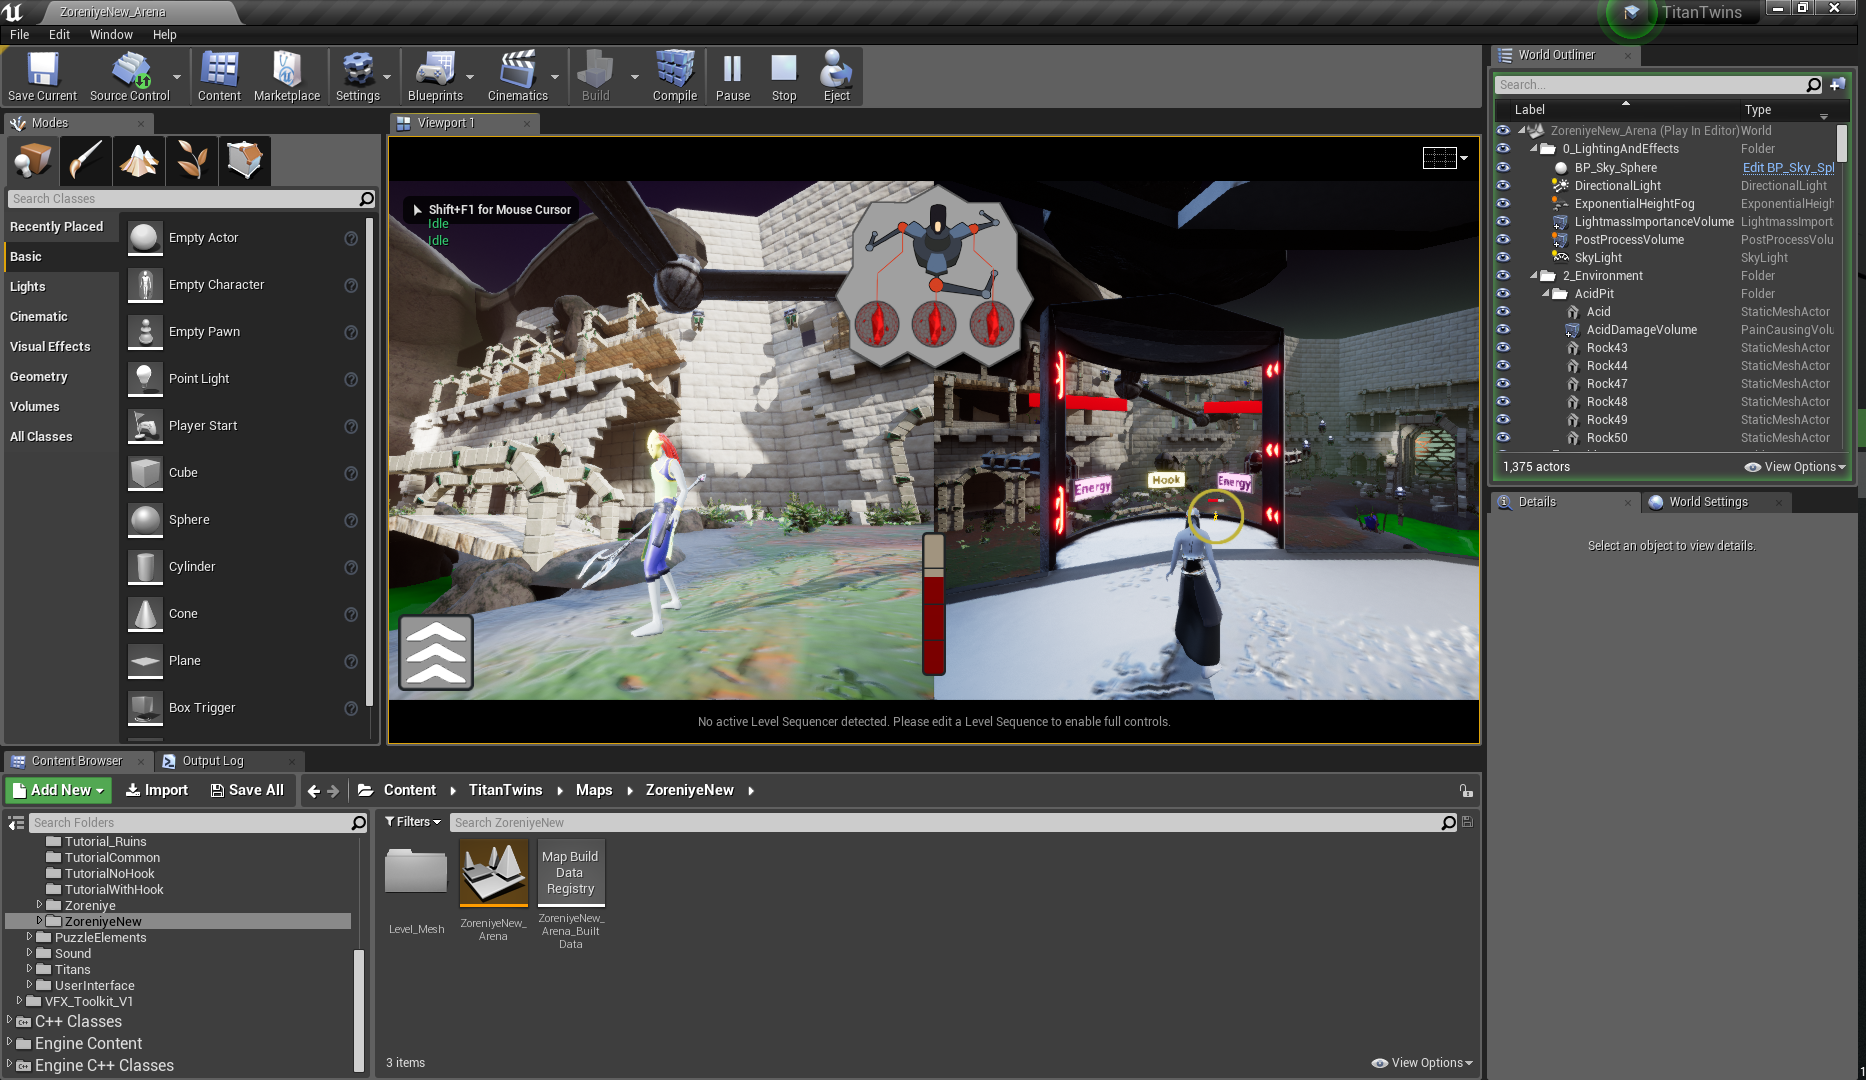
\includegraphics[width=\linewidth]{PICs/unreal_ed.png}
	\caption{The editor shipped with \ac{UE4}}
	\label{fig:unreal_ed}
\end{figure}

Going from left to right and top to bottom, Figure \ref{fig:unreal_ed} shows a selection for actors (objects that can be placed in the game world), a game world view, the world outliner (hierarchy of actors) and the content browser, that lists all folders and contained assets. The editor is a place where designers can create the game world, where artists can author special effects and their assets directly in the game
and where designers and programmers can develop the rules and logic needed to drive the world. For creating this logic \ac{UE4} offers two possible ways: scripting via the \textit{Blueprint} system or directly in C++. \ac{UE4} comes with the integrated \textit{Blueprint Visual Scripting} system that allows for gameplay programming using the concept of a node-based graph. This system is versatile and if it has reached it's capacities a programmer can still implemented the necessary or performance critical parts in C++ and expose an interface for the designer to use the component together with built-in blueprints.

\begin{figure}[h!]
	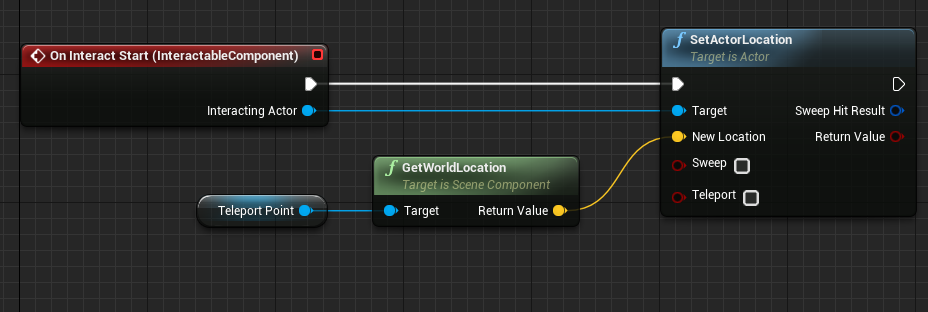
\includegraphics[width=\linewidth]{PICs/ue_blueprints.png}
	\caption{A very simple example that shows how the blueprint visual scripting looks like in \ac{UE4}}
	\label{fig:ue_blueprints}
\end{figure}

A very similar system of node-based graphs is used for building complex materials in \ac{UE4}. A material describes how an object, that uses it, looks like. It can for example define how it reacts upon light, whether the object appears to be rough or specular. The advantage of \ac{UE4}'s approach, using a node-based abstraction for materials, is that it makes life easier for developers when creating and authoring styles or effects. Without this system in place it would require a graphics programmer to write a shader. There are many different kinds of shaders but to keep it simple and because it is not necessary for now it is enough to say that a shader is a program that is executed on the \ac{GPU} and defines which color a pixel shall display at the end. Writing such shaders is not a trivial task. The node-based approach puts a layer of abstraction upon this process that allows developers to work with materials without needing to know the low-level internals of shaders.

It should not be unmentioned that working with \ac{UE4}, especially when needing very specific features or techniques that are not exposed to the abstraction systems, it requires a fond knowledge of C++ and the internal engine systems to fulfill the task. \ac{UE4} has grown in the past years and due to the fact that its source code is authored by many developers, both Epic engineers and open source contributors, bug reports are likely prioritized in relation to the needs Epic has for its own products developed in \ac{UE4}. The documentation is well written for engine tools and visual scripting but is a little weak on the C++ side. When working directly in C++ sometimes compile-times can decrease iteration times in \ac{UE4} which is due to the \ac{UBT} and some default configurations on how to deal with precompiled headers and unity builds.

To conclude this paragraph about \ac{UE4} it can be said that Epic created an engine that is suitable for creating games from any genre, which sometimes require tweaking the engine's source code. \ac{UE4} offers a variety of tools and integrations for asset authoring software which makes it easy for developers to start working with it. The abstraction systems paired with the revenue share licensing model lowered the entrance barrier for new game developers and are a reason for why the engine is in such a good market position. The development experience and fast iteration times fade away the more direct C++ coding is involved but again a trade-off between developing every system in-house and dealing with problems that rise has to be made.

\subsection{Unity}

The biggest competitor on the market for \ac{UE4} is Unity, and there are several reasons why there is a second product that viable. Unity was born in 2004 and created by the company called \textit{Over the Edge} which was later re-branded to \textit{Unity Technologies}. Contrary to the evolution of \ac{UE4} that evolved from moddable games and with easy extension in mind, Unity was created to lower the access barriers for 2D and 3D game development. After their first game, GooBall, failed commercially the founders discovered how valuable engine software and tools are. This led to their decision of building an engine that is accessible to as many people as possible and that promises ease of development and cross-platform support. With these principles in mind Unity became a product that was adopted by many developers and nowadays is used by many studios and small developers.

In contrast to \ac{UE4} the source code of Unity is not freely accessible but it can be acquired by acquiring an enterprise subscription. If source code access is not needed, which is the case more a major percentage of the developer products, Unity offers a very fair licensing model. A personal license can be registered for free, with the constraint that a product does not generate more revenue than 100.000\$ annually. This version includes all Unity core features as well as continuous upgrades and access to Unity beta versions. The next tier, called Unity Plus, includes everything of the previous one and adds more flexible customizations (custom splash screen, pro editor UI), more in depth analytics and it alters the cap of concurrent players on multiplayer games hosted by Unity. The Plus tier costs 35\$ per month and is constrained by a revenue cap of 200.000\$ per year. If the income exceeds that limit, the Unity Pro tier comes without any revenue limit at all for 125\$ per month. It adds again more in-depth analytics and alters the concurrent players cap once more.

Independent of the selected tier, Unity includes an editor to interact with its tools and the game world. 

\begin{figure}[h!]
	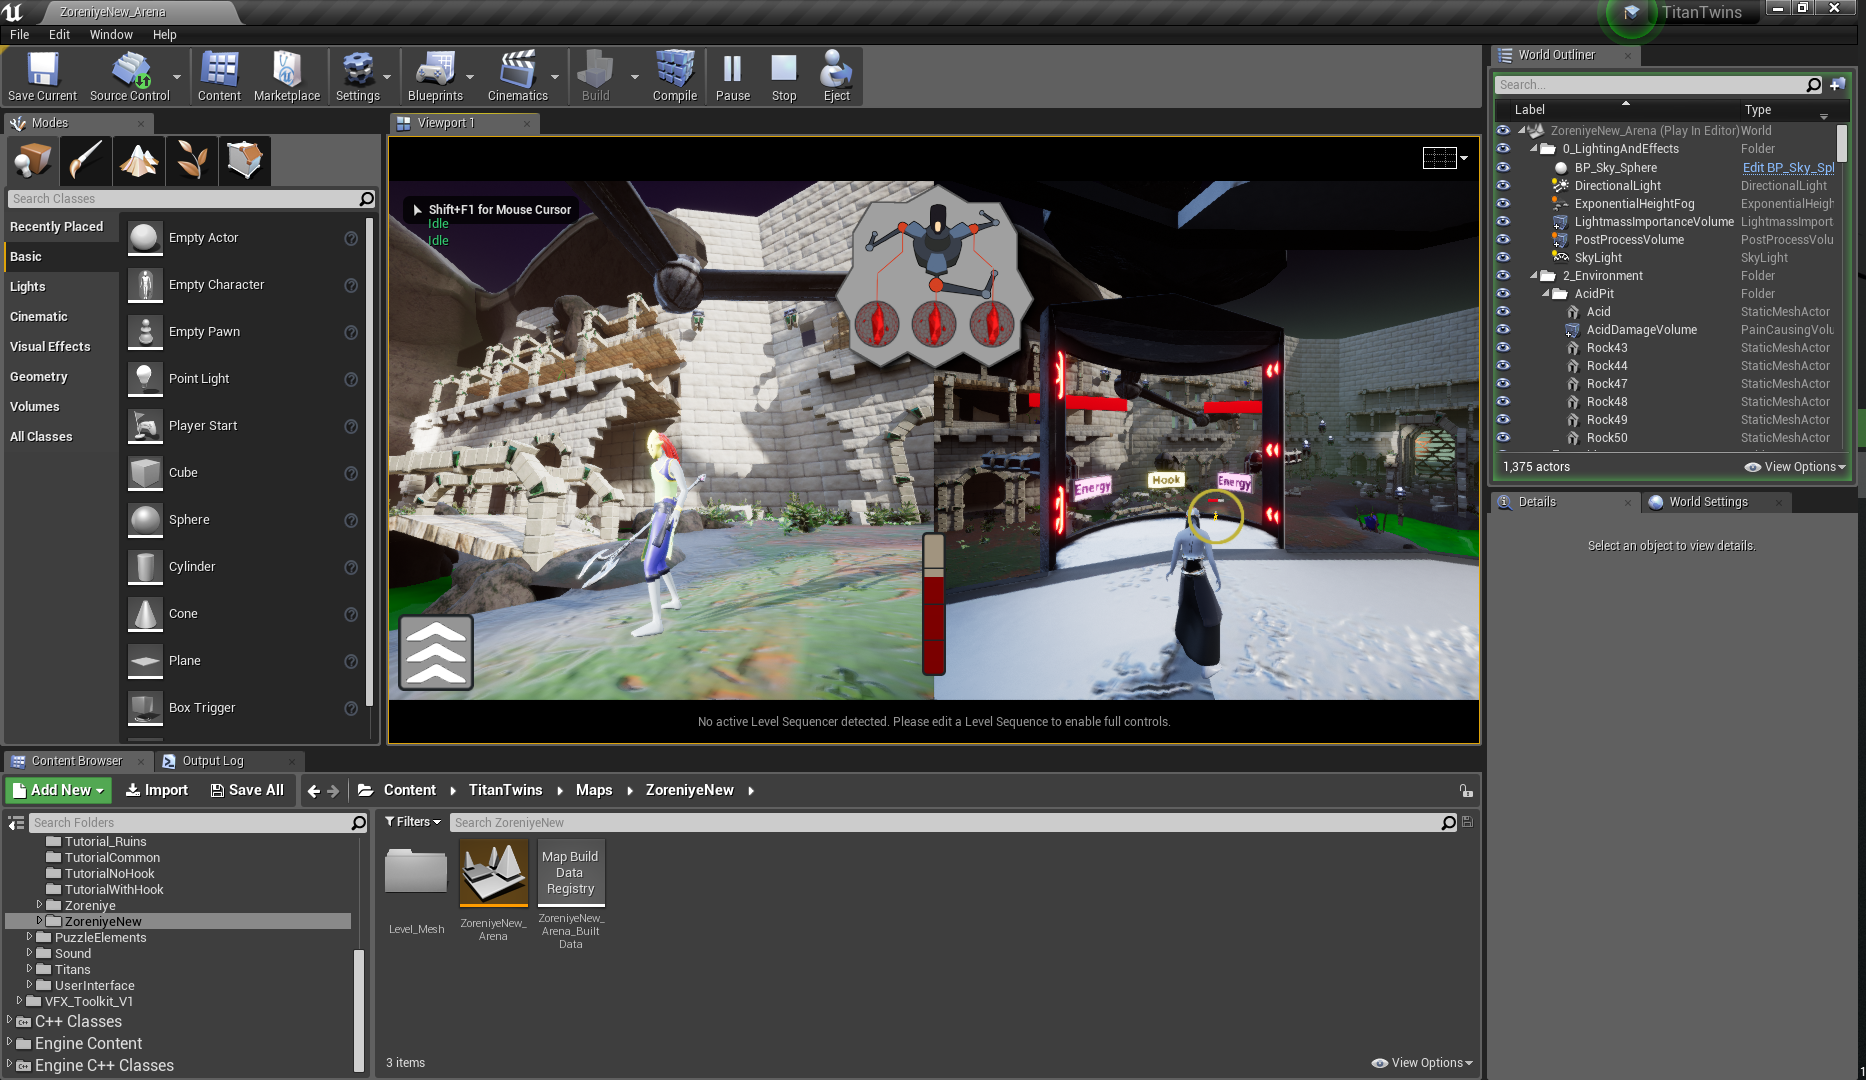
\includegraphics[width=\linewidth]{PICs/unreal_ed.png}
	\caption{The default layout of the editor shipped with Unity}
	\label{fig:unity_ed}
\end{figure}

The editor is quite similar to the one of \ac{UE4} but the views and tools differ in their naming. Going from left to right and top to bottom Figure \ref{fig:unity_ed} shows the Hierarchy, collection of game objects that are placed in the game world, the scene or current world, the Inspector, a list of components attached to a single game object and the project structure showing folders and assets. 
What was called an actor in \ac{UE4} can be compared to a game object in Unity. A game object is an entity that can be placed in the world but does not contain any logic itself. Rather it is a container that holds a collection of components, each holding data or logic. This system of entities and components is called an \acl{ECS} and will be described in detail at the end of this chapter. Because of the \ac{ECS} components can be shared and reused among projects which simplifies the development process and cuts iteration times when done properly.
It was already mentioned that components can also contain logic which already describes the basics on how game rules and logic are created in Unity. Where \ac{UE4} provides a visual scripting system Unity does not have anything similar. In Unity scripting is done in C\#, a high-level programming language running in the MonoDevelop/.Net runtime. The work flow of creating gameplay logic often starts with a programmer creating a new scripting component in C\# which then later can be used by designers to assemble new game objects without needing to touch any C\# code. This is ensured by a system that allows programmers to expose certain properties of the script to the editor, where values can be tweaked by designers to fit the needs of the game. Although Unity does not have a visual scripting system it is easy to create scripts because they are contained withing a single component and an error inside of them will not crash the whole engine but is guarded by the scripting runtime.

\subsection{Molecular}
\blindtext
\subsection{Tombstone}
\blindtext
\section{Rust game engines}
\blindtext
\subsection{Piston}
\blindtext
\subsection{Amethyst}
\blindtext
\section{Tools and asset pipeline}
\blindtext
\subsection{Editor}
\blindtext
\subsection{Asset pipeline}
\blindtext
\section{Engine subsystems overview}
\blindtext
\subsection{Memory Management}
\blindtext
\subsubsection{Custom Allocators}
\blindtext
\subsection{Job System}
\blindtext
\subsection{Rendering}
\blindtext
\subsection{Entity Component System}
\blindtext
\subsection{Scripting}
\blindtext